\documentclass{article} 
\usepackage{geometry,graphicx,float}
\geometry{
	a4paper,
	total={170mm,257mm},
	left=20mm,
	top=20mm,
}
\linespread{1.5}
\title{Predicting Gene ``Mapk1" in Mice}

\author{
  D'Azevedo, Gloria\\
  \texttt{gad87@cornell.edu}
  \and
  Yadav, Pihu\\
  \texttt{py82@cornell.edu}
}
\date{December 2, 2016}

\begin{document}
\maketitle

\section{Executive Summary}
%This needs to be written last

\section{Introduction and Problem Definition}
The goal of this analysis is to take a gene expression data set for a mouse and develop a model to predict the amount of the gene ``Mapk1".  This gene is very prominent and plays a significant role in cell proliferation.  In general, cells reproduce to make new healthy cells and dispose of older cells; however, an abnormally large amount of cell proliferation can lead to cancerous cells.  If there exists a good (cheap and fast) method to measure the gene creation of proliferating proteins in a patient over time, then the doctors can detect the early onset of cancer and other diseases.  Early diagnosis and the resulting less-invasive treatment usually result in higher survival rate for these patients.  Gene tests in the present day can generally be run to measure the amount of a specific gene in a sample; however, the process can take up to a few days and a sample can only be used once to test the amount of a gene, reliably.  Thus, the goal is to find a model that can accurately predict the amount of the gene  ``Mapk1" with the fewest number of predictors, or other gene tests.\\
\null\\
%
In general, gene analysis is important because they are an indicator for the current and future health issues for the organism as well as the organism's offspring.  However, the procedures to decompose the gene expressions can be expensive and can take a long time, so a model that requires few predictors to predict the value of a certain gene is crucial to accurate and early diagnosis for a potential disease.  In addition, experiments can be done to assess the effects from the presence or absence of specific genes to an organism so cures for these diseases can be developed and doctors know exactly what genes to target to cure their patients.\\
\null\\
%
The data set that is used to develop a model is very small.  There are only 40 different gene expressions, with the responses from 24 genes
in each.  There are no missing values.  The responses are all real numbers, ranging from -2.5 to 2.  Model types to investigate include best subset selection and forward/backward selection for linear model selection (with least squares as the loss function) as well as regularized linear regression.  In addition, resampling methods such as boostrapping and cross-validation will be extremely useful as there is so little data.  These methods and techniques are generally quite interpretable and the robustness can be tested using the resampling methods mentioned above.\\
\null\\
In addition, for model size selection we use the Bayesian Information Criterion as a measure of model fit that takes into account model size.  The function to calculate the BIC is as follows:
\begin{equation}
BIC=-log(L)+d*log(n)
\label{eq:BIC}
\end{equation}
In Equation \ref{eq:BIC}, $L$ is the value of the likelihood function, $d$ is the number of predictors in the model, and $n$ is the number of data samples.  A smaller value of BIC implies a better model fit.  \\
\null\\
After choosing the correct number and set of predictors, we use non-regularized regression (calculated via least squares) to calculate the coefficients for each of the predictors and evaluate the fits of those using the Adjusted $R^2$ metric which measures how good the data fits to a linear model but also taking into account the size of the model.  The exact calculation of Adjusted $R^2$ ($R^2_{adj}$)is as follows where $R^2$ denotes the non adjusted $R^2$ and can be found below in Equation \ref{eq:R2}.
\begin{equation}
R^2_{adj} = R^2-(1-R^2)\frac{p}{n-p-1}
\label{eq:AdjR2}
\end{equation}

\begin{equation}
	R^2=1-\frac{\sum_{i=1}^n (y_i-\hat{y_i})^2}{\sum_{i=1}^n (y_i-\bar{y})^2}
	\label{eq:R2}
\end{equation}
%
\section{Model Development}

\subsection{Best Subset Selection Using Linear Models}
There are 22 genes that can be leveraged to predict the response for the ``Mapk1" gene so one of the implemented models is the best subset selection algorithm.  In this algorithm, all possible $2^r$ linear models are fit to the data using least squares where $r$ is the number of predictors (in this problem, $r=22$).  Then, the algorithm returns the best set of predictors for a model of size $r$, for each $r$.  Generally, this algorithm is very computationally intensive but there are only $n=40$ data points so each iteration runs quite quickly on an average computer.  The downside of this algorithm for this data set is that there are only 40 data points, so splitting it further into training and test sets would yield poor estimates of the model for each iteration and the test set is still quite small.  In addition, there are more steps to fit each of the best predictor subsets to the data again to find the coefficients for the linear model of that size and to evaluate the training error and/or test error, if applicable.\\
\null\\
\begin{figure}[H]
	\caption{Best Subset of Predictors for Each Model Size, ordered by increasing BIC}
	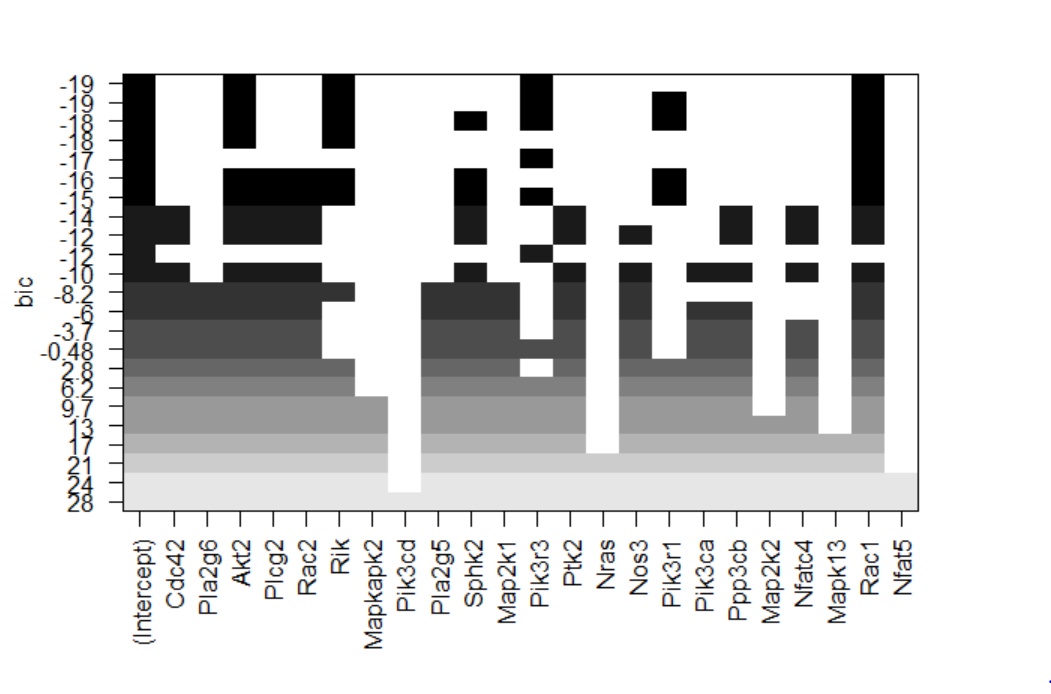
\includegraphics[scale=0.60]{best_subsets}
	\centering
	\label{fig:best_subsets}
\end{figure}
From the chart we determine that the model with the lowest BIC value is the one that includes $Akt2$, $Rik$, $Pik3r3$, and $Rac1$.  
\subsection{Forward-Backward Model Selection}
The Forward-Backward Model Selection is a variant of the Best Subset Selection which is less computationally expensive.  In the future, if we had more predictors or genes for the model instead of only 22, then this would be a good algorithm to use instead of best subsets as the number of models tested increases linearly instead of exponentially.  The algorithm starts with an initial model and a corresponding objective value (in this case we use the Bayesain Information Criterion (BIC) because it has a larger penalty on larger models).  For each step in the algorithm, models with one more variable than the current model and models with one less variable than the current model are each fit in turn and the BIC is calculated for each.  In other words, if the current size of the model was $k$, then the model fits $22-k$ models of size $k+1$ and $k-1$ models of size $k-1$ and evaluates the objective value of each.  The next step of the algorithm uses the model with the smallest objective value to proceed with the next iteration (which could be the original model of size $k$).  The algorithm finishes when adding or removing a variable from the model would yield a higher BIC value.\\
\null\\
When implementing the forward-backward model selection, we also included Leave-One-Out-Cross-Validation (LOOCV) to have disjoint training and test data.  Obviously if we had more data, then we would use a k-fold cross validation with 5 or 10 folds instead of $n$ folds which is how LOOCV is implemented.  Thus the whole procedure is as follows:\\
\null\\
For each $i=1,\dots, n$:\\
1. Use data point $i$ as the test set and the rest of the data as the training set.\\
2. Perform stepwise forward and backward selection using BIC as the objective value to minimize.\\
3. Calculate the test error using data point $i$. \\
Teh final optimal model using this method includes $Akt2$, $Rik$, $Rac1$, $Pik3r3$ as the predictors in the linear model.

\subsection{Linear Regression with Regularization}
As an extension to linear regression, we also incorporate a regularizer in order to make the model more robust and determine which predictors are the most significant.  In other words, instead of trying to find the coefficients for the linear model that minimizes the squared errors, we include some bias in the model in order to decrease the variance of the model and prevent overfitting.  This bias is of the model is shown by decreasing the coefficients of some predictors to be exactly $0$ which may not yield the smallest sum of squared differences, but for estimating new data the model will be more accurate. \\
\null\\
For this application, we would like to test and evaluate the fewest number of genes possible as the chemical processes can take a long time.  Thus, we prefer a sparse model so that fewer genes are needed to predict the response gene ``Mapk1" and a model with fewer predictors will have smaller variance.\\
\null\\
The lasso regularizer for linear regression yields sparse models.  When determining the coefficients for this model, we want to minimize the following objective function.  The rows of the input data are denoted by $x_i$ while the whole matrix that is used is $\mathcal{R}^{nxd}$, the output or response for data point $i$ is denoted by $y_i$ and the coeffecients for the predictors of the linear model are denoted in the vector $w$ that is made up of components $w_j$ for $j=1,\dots,d$
\begin{equation}
	\textbf{minimize}_w \sum_{i=1}^n(y_i-x_i^Tw)^2+\lambda\sum_{j=1}^d |w_j| = \textbf{minimize}_w \sum_{i=1}^n(y_i-x_i^Tw)^2+\lambda||w||_1
\end{equation}
For this problem with few data points, we use cross validation to find optimal $\lambda$ value which acts as measure of how much bias the model is able to have.  If $\lambda = 0$ then we get the nonregularized problem, however, if $\lambda$ is too large, then all of the coefficients will go to $0$ to find the minimum objective value.  The $\lambda$ that minimizes the mean cross validated error yields a model with 6 predictors and an intercept and the resulting mean squared error is 0.0121.  We also investigate using the largest $\lambda$ such that error is within 1 standard error of the minimum value of the response.  This yields a smaller model with an intercept and only 4 predictors and a corresponding mean squared error of 0.013. This value is not significantly different from the mean squared error of the $\lambda$ corresponding to the minimum mean squared error of 0.0121 so we still keep it in consideration if we want a simpler model with slight increase in the mean squared error.  The significant predictors from the simpler model are $Rik$, $Pik3r3$, $Rac1$, and $Nfat5$.  

\section{Results and Conclusions}
Because our outputs are real numbers, we use a squared error loss to evaluate the training error and the test error of our model but we also want to keep in mind that a simpler model is better even if we have to add some bias to decrease the overall variance of the model.  From the best subset regression, we see that the predictors for the model are $Akt2$, $Rik$, $Pik3r3$, and $Rac1$ (Model 1) when we do not use the $\lambda$ corresponding to the minimum mean squared error but instead use the maximum value of $\lambda$ that the mean squared error is still within a reasonable bound of the minimum mean squared error.  From the forward-backward subset selection with LOOCV, we get a linear model with the same 4 predictors as well: $Akt2$, $Rik$, $Rac1$, $Pik3r3$.  However, when using regularized linear regression, we see that we get a slightly different set of 4 predictors for the model: $Rik$, $Pik3r3$, $Rac1$, and $Nfat5$ (Model 2).  \\
\null\\
Investigating this discrepancy between the predictors in each of the models, we note that the gene $Nfat5$ is fairly positively correlated with $Rik$ (the correlation between them is 0.6033).  Thus, if the model includes the genes $Nfat5$ and $Rik$, then not much new information is being added.  Also we note that the response gene $Mapk1$ is strongly positively correlated with $Rik$ (their correlation is 0.5750) and also strongly positively correlated with $Pik3r3$ (their correlation is 0.6139).  Thus we suspect that these two genes are useful for predicting the amount of $Mapk1$.  Also, $Mapk1$ is strongly positively correlated with $Nfat5$ with a correlation of  0.5532 so we may be more inclined to use these 3 predictors in the model at least. \\
\null\\
Fitting a non regularized linear model to each of the aforementioned Models 1 and 2, we get the following equation:
\begin{equation}
	Mapk1 = -0.44461-0.40548Atk2+0.22072Rik+0.24399Pik3r3+0.31716Rac1
	\label{eq:Model1}
\end{equation}
All the predictors in Model 1 are significant to the model, and $R^2_{adj}=0.5656$.\\
\null\\
For Model 2 we get the following equation:
\begin{equation}
	Mapk1=-0.3109+0.1741Rik+0.2331Pik3r3+0.2570Rac1+0.0864Nfat5
	\label{eq:Model2}
\end{equation}
However in Model 2, only $Rac1$ is singificant to the model at the 0.001 significance level and $Pik3r3$ is significant at the 0.1 significance level.  In addition, $R^2_{adj} = 0.4998$ which is smaller than that of Model 1.\\
\null\\
We also note that even with a model of only 4 predictors, we are decreased to only 35 degrees of freedom since we need to estimate the coefficients for each of the 4 predictors as well as the intercept for the linear model.  Since there are so few degrees of freedom, we may instead want to assume that the errors are from a student-t distribution instead of a normal distribution to get a more conservative estimate.

\section{Next Steps}
In the future, if data is collected for more mice and there are more gene expressions to analyze, other methods such as K-Nearest-Neighbors (KNN) can be implemented which is a robust, unsupervised machine learning technique.  Currently, as there are only $40$ 
samples, the number of points that have k nearst neighbors is at most $40-k$, assuming that the whole data set is used as a training 
set and none of it is used to evaluate the model and estimate test error.  Currently if the algorithm is implemented, the 
model is grossly overfit on the training data, which yields a low training error, which does not imply a low test error for future samples.\\
\null\\
In addition, in the diagnosis setting, there may also be predefined ranges of the amounts of the gene or protein that can be a normal range, a warning range, and a dangerous range of that gene or protein.  In that case, we can reframe the problem as ordinal classification and use methods such as KNN, decision trees, or other machine learning techniques.  These methods are more variable and some sort of resampling method will still have to be used since there is not much data present. 
\end{document}